%#BIBTEX pbibtex aiit_bulletin
%% 産業技術大学院大学紀要フォーマット
%% Created: 2013-06-30 Y.Chubachi
\documentclass[a4j, 12Q, twocolumn, twoside]{jsarticle}
\usepackage{aiit_bulletin}		% 紀要のスタイル

%%
%% 1.必要に応じてパッケージやマクロをここに追加
%%
\usepackage{newcent}			% Centuryフォント
\usepackage[dvipdfmx]{graphicx}		% 図の取り込み(PDF対応)用
\usepackage{okumacro}			% ルビ・圏点など
\usepackage{url}			% URLの出力

%%
%% 2.英語論文の場合は下記2行のコメントを外してください
%%

% \renewcommand{\tablename}{Table~}
% \renewcommand{\figurename}{Fig.~}

%%
%% 3.タイトルを設定してください
%%
%% 本文が英文の場合は,\etitle, \eauthorを削除し,\titleと\autherに
%% 英文を記入してください.
%%

%%
%% 和文表題
%%
\title{ロボットサービスの国際開発プロジェクトモデルにおける\\
アジャイル型ソフトウェア開発プロセスScrumの適用}

%%
%% 和文著者名
%%
%% \thanksの中で改行する場合\\ではなく\newlineを使用する
%%
\author{
  酒瀬川 泰孝
  \thanks{産業技術大学院大学 \newline
  Advanced Institute of Industrial Technology}
  木崎 悟
  \thanks{電気通信大学 \newline
  The University of Electro-Communications}
  川木 富美子
  \thanksmark[1]
  須澤 秀人
  \thanksmark[1]
  \\
  Truong Anh Hoang
  \thanks{ベトナム国家大学ハノイ校 \newline
  Vietnam National University, Hanoi}
  Thi-Minh-Chau Tran
  \thanksmark[3]
  \\
  土屋 陽介
  \thanksmark[1]
  加藤 由花
  \thanksmark[1]
  中鉢 欣秀
  \thanksmark[1]
}

%%
%% 英文表題
%%
\etitle{Applying Agile Project Management with Scrum\\
for International Robot Service Software Development Projects}

%%
%% 英文著者名
%%
\eauthor{
  Yasutaka Sakasegawa
  \thanksmark[1]
  Satoru Kizaki
  \thanksmark[2]
  Tomiko Kawaki
  \thanksmark[1]
  Hideto Suzawa
  \thanksmark[1]
  \\
  Truong Anh Hoang
  \thanksmark[3]
  Thi-Minh-Chau Tran
  \thanksmark[3]
  \\
  Yosuke Tsuchiya
  \thanksmark[1]
  Yuka Kato
  \thanksmark[1]
  Yoshihide Chubachi
  \thanksmark[1]
}

%%
%% 英文アブストラクト
%%
\begin{abstract}
Globalization progresses accelarative and offshore development is
increasing.  In robot service software development, it is required that
engineers have to develop various requirement specifications quickly in
an international development project.  However, it is also a fact that
there is no effective development process of international robot
service, and this fact has been a subject of the development project.
We created the new development model based on project management using
the agile development with scrum which is the knowledge from software
engineering.
\end{abstract}

%%
%% 英文キーワード
%%
\keywords{Robot Service Software Development,
Agile Project Management, Scrum,
International Project Based Learning}

%%
%% 受領日
%%
\receivedon{2013-09-30}

\begin{document}
%%
%% 4.タイトルを出力
%%
%% \maketiteleにあるオプション[0pt]はタイトルと本文の間隔
%% を調整するものです.
%% 1ページ目の脚注の下端と本文の下端が左右の段で揃わない
%% とき,この値を0pt〜8ptくらいの範囲で調整してください.
\amaketitle[-1pt]

%%
%% 5.本文
%%
%% 本文
\section{はじめに}

ロボットを用いて新たなサービスを実現するためには,
付随するソフトウェアを迅速に開発することが求められる.
このためには,ロボット工学の知見に,最新のソフトウェア工学を融合させることが必要となる
%###
\cite{pons2012systematic}
%###
.
一般的に,ソフトウェア開発のプロセスとしてウォーター・フォール・モデルが広く知られている.
しかしながら,このモデルはロボット開発には不適当であり,
より新しい反復型の開発プロセスを利用するのが良いとされる
%###
\cite{kaindl2009iterative}
%###
.

一方,ソフトウェア産業界においても,
迅速な開発スピードや,顧客からの要求事項の変化に強いという理由から
アジャイル型の開発プロセスが普及しつつある.
特に,
J.Sutherlandが,ソフトウェア開発プロセスとして体系化したScrum
%###
\cite{sutherland2008agile, sutherland2011scrum}
%###
は,竹内・野中による日本の製品開発におけるベストプラクティスに関する研究
%###
\cite{takeuchi1986new}
%###
が基礎となっているため,
日本人にも取り組みやすい開発方法論として注目されている.

\begin{figure}
  \begin{center}
    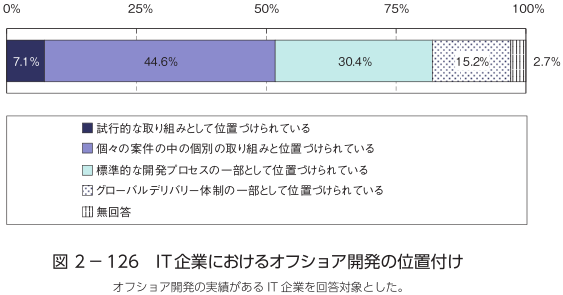
\includegraphics[width=\columnwidth]{./figures/IT_Jinzai.png}
    \caption{Off-shore developments in IT companies}
    \label{fig:itjinzai}
  \end{center}
\end{figure}

加えて,近年のソフトウェア産業界の動向として,
開発コストを低減することを目的とした,海外へのアウトソーシングも一般的になっている.
独立行政法人情報処理推進機構(IPA)発行のIT人材白書2012
%###
\cite{IT人材白書2012}
%###
によると図\ref{fig:itjinzai}に示す通り
オフショア開発経験のあるIT企業のうち45.6%の企業が組織的にオフショア開発に取り組んでいる.

これらのことから,今後は,ロボット・サービスの開発においても,最先端の
ソフトウェア工学の知見に基づき,海外の技術者とも連携しながらサービスの
開発をするプロジェクトが増えてくると予想する.同時に,このような開発モデ
ルに対応できるソフトウェア技術者の教育の必要性も高まってくる.

\begin{figure*}
  \begin{center}
    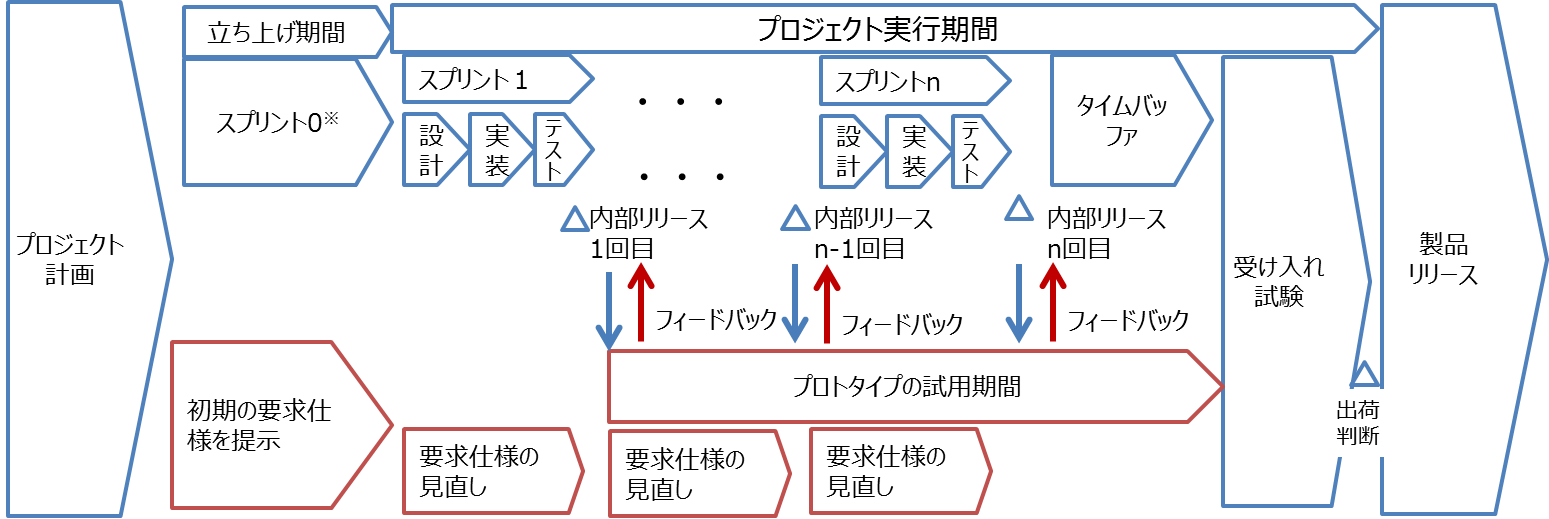
\includegraphics[width=\textwidth,trim=0mm -5mm 0mm 0mm, clip]{./figures/Process.png}
    \caption{Overall Process of New development Model}
    \label{fig:OverallProcessofNewdevelopmentMode}
  \end{center}
  %\label{fig:新国際開発プロジェクトモデルのプロセス全体像}
\end{figure*}

そこで,本論文ではロボット・サービスの開発を目的としたアジャイル型のソ
フトウェア開発プロセスを,海外の技術者と共同で開発するための開発プロセ
スモデルを提案する.これを,産業技術大学院大学のプロジェクト型学習
(PBL: Project Based Learning)においてベトナム国家大学の学生との国際的
なロボット・サービスに適用して得られた知見を報告する.以下,
\ref{sec:background}章で研究の背景と関連研究を示す.\ref{sec:model}章で
ロボット・サービス開発に適した新しいソフトウェア国際開発プロジェクトモデルを定義し,
\ref{sec:result}章では本モデルをPBLにおいて利用した結果について記す.
\ref{sec:lessonslearned}章では,本プロジェクトで得られた知見を整理し,
このモデルの有用性を示す.最後に,\ref{sec:concludion}章でまとめを述べ
る.

\section{関連研究}\label{sec:background}
近年,大学生を対象としたプロジェクト型教育においてScrumを適用する事例
が増えている
\cite{mahnic2012capstone,mahnic2012students,wagh2012using,devedzic2011teaching}
.特に,LEGO MINDSTORMを使ったPBLにおいてScrumを適用した例として文献
%###
\cite{pinto2009useofscrum}
%###
があり,プロジェクトのマネジメントに効果があるとの指摘がある.しかしな
がら,外国との国際的なプロジェクト型学習に対してScrumを適用した事例は見
当たらない.国際的なプロジェクトを通したソフトウェア工学教育の事例とし
ては,文献\cite{de2006germany}が報告されている.

産業技術大学院大学(AIIT) \footnote{AIITは専門職大学院であり,学生の大多
数が社会人である.PBLは学生の専門的業務遂行能力の向上のために,通常の修
士論文と同じ位置付けで,カリキュラムにおける中核的な教育手法として導入
している.}ではベトナム国家大学ハノイ校(VNU)の学生と共に国際PBLを実施し
ている
%###
\cite{pub:tozawa-global-2009,大類優子2009n,nishino2010,木崎2011チケット駆動}
%###
.


%
2011年度より,ソフトウェア開発プロセス教育の一環としてLEGO
MINDSTORMSによるロボット・サービスの開発をテーマとして取り上げている
%###
\cite{木崎悟2012国際}
%###
.
%
特に,2012年度は,ソフトウェア部分の開発プロセスとしてScrumを全面的に採
用し,VNU側学生への開発プロセス教育を含むロボット・サービス開発プロジェ
クトを実施した.これらを通し,海外とのPBLにおいて発生する課題や,解決策
に関する知見が得られている.

IT人材白書2012\cite{IT人材白書2012}にもある通り,ソフトウェア開発におけ
る海外へのアウトソーシングにおいては,言語が異なることによるコミュニケー
ションの難しさと,相対的な品質の低さが大きな問題である.海外との国際的
なロボット・サービス開発に対応した国際開発プロジェクトモデルを新たに定義し,PBLを中心と
した技術者教育の手法とあわせて提供することで,これらの課題の解決をはか
ることができる.



\section{ロボットサービス開発に適した国際開発プロジェクトモデル}\label{sec:model}
\subsection{国際開発プロジェクトモデルの概要}

Scrumは少人数(5人から9人程度)の単一チームで単拠点,短期間にソフトウェ
ア開発を行うことを前提とした開発手法である.これを,国際的なプロジェク
トに適用するためには,国際開発の体制やマネジメントプロセスを追加する必
要がある.

そこで我々は,国際開発プロジェクトに適用できる,Scrumをベースとした新た
なモデルを提案する.図\ref{fig:OverallProcessofNewdevelopmentMode}に
その全体像示す.プロセスの拡張はスプリントの追加という形で行い,以下,
拡張したポイントについて説明する.

\begin{description}
 \item[スプリント0(準備スプリント)] 国際開発における開発上のリスクを前
	    もって低減させるために実施するものである.この期間では,重要
	    な要件の洗い出しやプロトタイピング,ツールのセットアップ等を
	    行い,スムーズに開発に入るための準備を行う.
 \item[受け入れ試験スプリント] オフショア開発における品質を確保するため
	    最終成果物リリース前に受け入れ試験スプリントを置き,品質管
	    理活動を開発プロセスに組み込む. 受け入れ試験スプリントでは
	    顧客の要求に基づく動作確認を行い,リリース可能な品質が確保
	    されているか確認する.
\end{description}


% \subsection{クリンナップスプリント}
% 品質向上のための工夫取りこぼしたバグの改修(掃除それぞれのスプリントで開発した機能の結合テスト,回帰テストなどを実施する.
また,Scrumを海外と国内の2つの拠点で実施するために,各拠点とその役割を次の通り定義する(図\ref{fig:organization structuree}).

\begin{description}
 \item[マネジメント拠点] マネジメント拠点の役割は,管理監督では無く,
	    開発拠点のメンバに対してプロジェクトの円滑な進行をサポー
	    トする支援機能を提供する.
 \item[開発拠点] それぞれの開発グループのメンバは,スクラムの自己組織
	    化のコンセプトに基づき開発作業の決定権を開発チームに委任し
	    自律性を重視した開発を実施する.開発拠点のチームのマネジメン
	    トはスクラムマスタに委任する.
\end{description}

% \begin{enumerate}
% \item 要求仕様の割り当てと調整
% \item 組織全体のプロジェクトマネジメント
% \item 開発が円滑に実施されるよう開発グループを支援
% \item ステークホルダとのコミュニケーション
% \item プロジェクトのモニタリング
% \item 品質保証活動
% \end{enumerate}

\subsection{コミュニケーションや共同開発のツール活用}

\begin{table}[h]
  \caption{ツール}
  \label{tb:Tools}
  \begin{center}
   \small
    \begin{tabular}{|p{6zw}|p{10zw}|p{10zw}|}
      \hline
      ツール & 用途 & 効果 \\
      \hline
      Skype\cite{Skype} & テレビ会議 & 会話を通した相互理解 \\
      Facebook\cite{Facebook} &時間と距離の制約の無いオンラインコミュニケーション &コミュニケーションの円滑化 \\
      Googleドキュメント\cite{googledocument} & 資料を共有し,タスク管理,進捗管理,課題管理 & 作業の見える化,成果物の見える化 \\
      GitHub\cite{GitHub} & 多拠点にまたがる構成管理 &統合開発環境Eclispeとの連携により効率のよいチーム作業が可能 \\
      \hline
    \end{tabular}
  \end{center}
\end{table}

\begin{figure}[htb]
%  \begin{minipage}{0.5\hsize}
  \begin{center}
   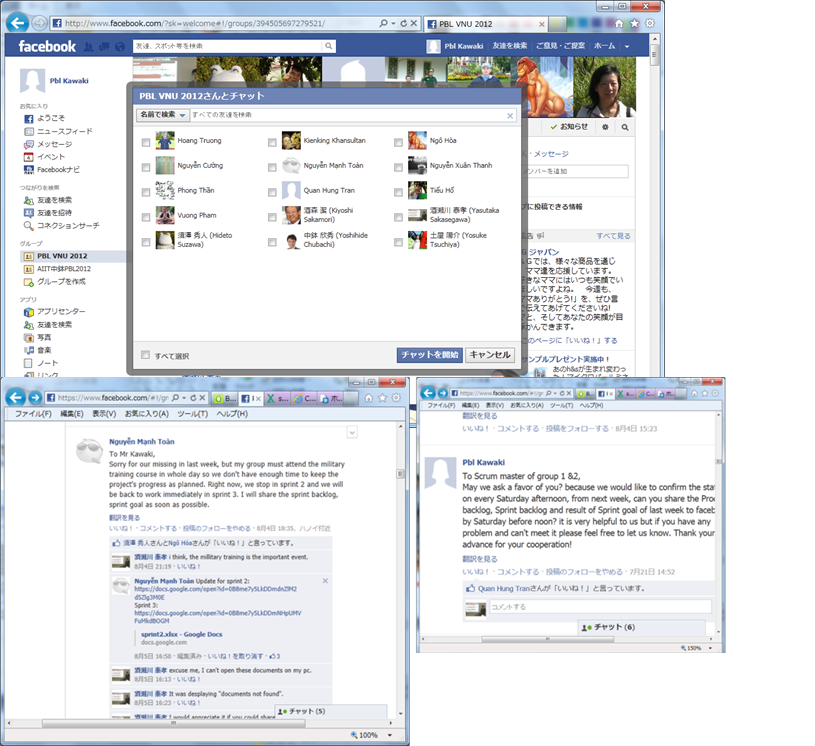
\includegraphics[width=\columnwidth]{./figures/SNS.png}
   \caption{SNS}
   \label{fig:SNS}
  \end{center}
%  \end{minipage}
%  \begin{minipage}{0.5\hsize}
%   \begin{center}
%    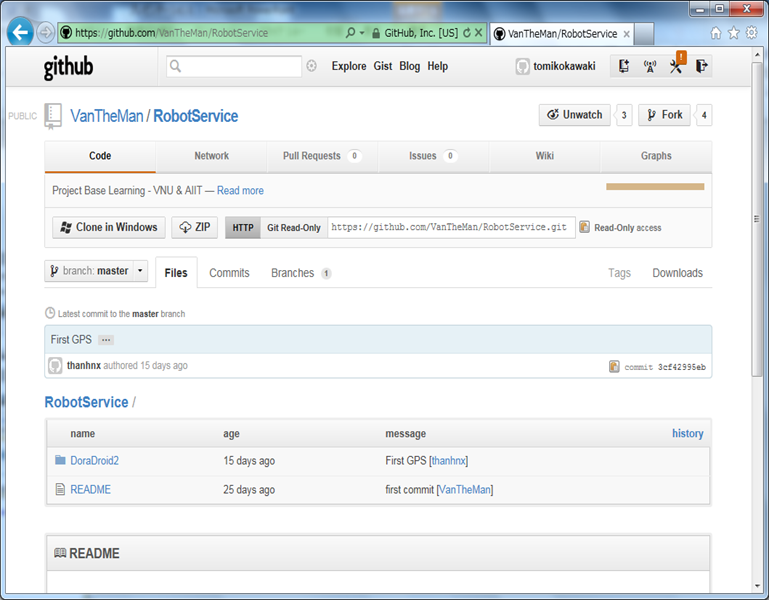
\includegraphics[width=0.8\columnwidth]{./figures/Github.png}
%    \caption{GitHub}
%    \label{fig:GitHub}
%   \end{center}
%  \end{minipage}
\end{figure}


本モデルは時差と距離を乗り越えながら,コミュニケーションをとるために,
表\ref{tb:Tools}に示す各種のソーシャルメディアやSkype等のツールを
用いる.
図\ref{fig:SNS}
にこれらのツールを利用している様子を示す.

ソーシャルコーディングのためのクラウド型ツールであるGitHub
% (Fig.\ref{fig:GitHub})
を用いることで,ソースコードの共有が円滑になる.この
ツールを用いることでメンバ全員がソースコードを参照したり,コメントし
たりできるようになる.

これにより,開発拠点におけるチーム全員誰もがソースコードを確認でき,問
題があればコメントすることでソースコードの品質を向上が期待できる.また,
マネジメント拠点における品質保証活動も容易にする.GitHubにあるソース
コードを日々チェックすることでソフトウェアの品質や技術的な課題の有無を確認できる.もし問
題があれば,直ちにコミュニケーションをとり,問題の解決を行う.

\subsection{その他の改良点}

\subsubsection{プロジェクト全体の進捗のモニタリング方法}
プロジェクト全体でバッファー(通常は各作業に積まれる不確実性に対応する
ための時間的な余裕)をプロジェクト全体で共有することで,遅延を見える化
する.本モデルでは「タイムバッファ」として取り入れる.

加えて,作業開始から現時点までに実施した作業量で進捗を管理するのではな
く,現時点から作業完了までの残り時間で進捗を管理することで,プロジェク
ト完了予定日と工期遅れの兆候を把握するようにする.

\subsubsection{国際開発でプロジェクトの全体を統合し支援するマネジメントの仕組み}
プロジェクトマネジメントやサポート機能をマネジメント拠点へ設置する.

自己組織化されたチームが生産性を高めるというスクラムの考えに基づき開発機
能はすべて開発拠点へ集約する.

オフショア先のメンバがプロダクトオーナーになることで,異言語のコミュニ
ケーションの難しさを排除する.

加えて,現場でプロダクトオーナーが作業の成果をチェックすることで品質低
下を未然に防くためである.

\begin{figure}[htb]
  \begin{center}
    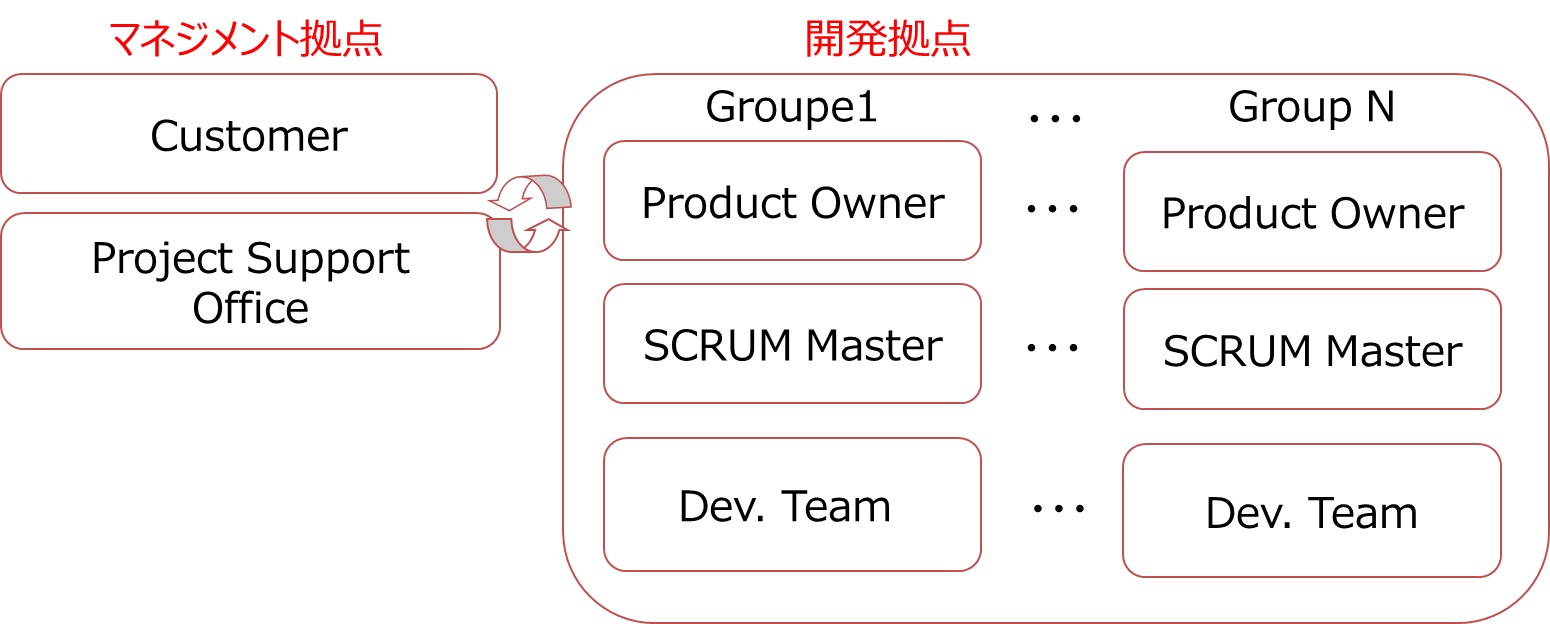
\includegraphics[width=\columnwidth]{./figures/organization_model.png}
    \caption{organization structure}
    \label{fig:organizationstructure}
  \end{center}
\end{figure}

\subsubsection{要求仕様の変更に対するリスク低減と生産性の両立}
要求仕様の変更は不可避なものと考える.
変更は開発者のモチベーション(生産性)を下げることにつながるので,スプリント期間中は変更認めない.
もし変更があった場合は次回以後のスプリントで取り込むこととする.
変更を次回のスプリントへ取り込むかどうかを要求仕様の優先度で判断できるため,
結果として要求や仕様の変更に柔軟に対応することと開発グループの生産性の両立が出来る


\section{国際開発プロジェクトモデルの試行結果}\label{sec:result}
\subsection{AIIT-VNU国際PBLの概要}
AIITおよびVNUとのグローバルロボット開発PBLで国際開発プロジェクトモデルの試行をした.
期間は2012年6月中旬から2012年8月末日までの約2カ月半のプロジェクト.参加メンバはAIITの院生とVNUの学生で構成された.
プロジェクトは以下の2つのフェーズから構成されている.

\begin{description}
\item[フェーズ1] アジャイル開発手法スクラムの教材開発とVNUにおけるオンサイトトレーニング
\item[フェーズ2] AIIT-VNU国際PBLロボットサービスソフトウェア開発プロジェクト
\end{description}

PBLで実施するロボットアプリケーション開発グローバルプロジェクトの成果
物は,RSNP
%###
\cite{narita2011enhanced,kato2011rsi}
%###
を利用したロボット・サービスとした.インターネット経由でアンドロイド端
末とLEGO MINDSTORMSを利用したロボットを操作するアプリケーションを開発す
る.そして,RSNPコンテストへ出場することとした.

表\ref{tab:GlobalPBL}にAIIT-VNU国際PBLの概要を示す.

\begin{table}[htb]
  \caption{国際PBLの概要}
  \begin{center}
   \small
    \begin{tabular}{|p{6zw}|p{20zw}|}
      \hline
      要員 & AIIT側:3名 (社会人大学院生:外資系ITエンジニア,ITインストラクタ,SI企業のPM) \\
       &VNU側: 学部3年生4名と4年生6名の計10名,各種プログラム言語既習,チーム開発経験無し \\      \hline
      期間 &2ヶ月 2012年7月~2012年8月 \\      \hline
       オンサイトトレーニング & 12(h)6時間×2日間\\      \hline
      キックオフミーティング &4 (h) \\      \hline
            ツール &開発ツール:Eclipse + Android SDK\\
& マネジメントツール:プロダクトバックログ,スプリントバックログ,バーンダウンチャート\\
&コミュニケーションツール:Skype\\
      \hline
    \end{tabular}
     \label{tab:GlobalPBL}
  \end{center}
\end{table}


\subsection{ロボットサービスの概要}
RSNPサーバーは,クラウドシステムであるAWS(amazonクラウドサービス)またはAIITのキャンパスに配置する.
WebブラウザでRSNPサーバにアクセスすることでLEGO MINDSTORMSロボットの操
作ができる.

ロボット側のアプリケーションはAndroidアプリとして開発する.
スマートフォンとLEGO MINDSTORMSロボットはBluetoothで接続する.
サーバは3G回線を通してインターネット経由で通信する.

\subsection{要求仕様}
顧客役のAIITの教員からは,
以下の優先順位と要求仕様でロボットの機能を開発するようにオーダーが出された.
\begin{enumerate}
\item RSNPサーバにHTTP接続したブラウザから,ロボットの動作制御(前進,後退,右折,左折,停止)ができる.
\item RSNPサーバにHTTP接続したブラウザから,アンドロイド端末に内蔵されたカメラを操作.画像はサーバに転送され,サーバ側ブラウザで確認できる.
\item RSNPサーバにHTTP接続したアンドロイドフォンから,GPS情報(緯度,経度)を取得し,インターネット経由でブラウザに表示する.
\end{enumerate}

\begin{figure}[htb]
  \begin{center}
    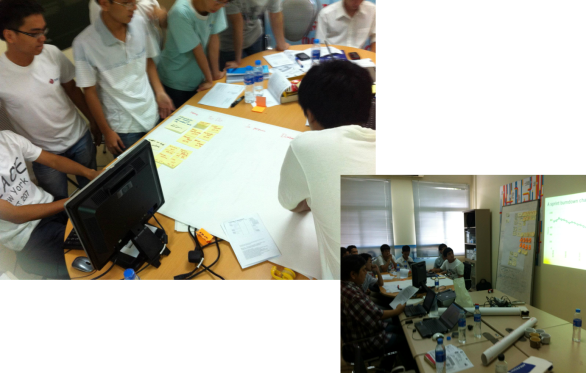
\includegraphics[width=\columnwidth]{./figures/training.png}
    \caption{Scrum Training}
    \label{fig:training}
  \end{center}
\end{figure}

\subsection{開制約条件}
制約条件として下記をプロジェクトに課した.
\begin{enumerate}
\item 時間と距離を克服し,VNU側の学生と協調しながら開発すること(グローバル).
\item 開発期間は,2ヶ月で固定の超短期開発(スピード・短納期).
\item RSNPロボットコンテスト出場可能なレベルのロボットアプリケーションを開発する(品質).
\end{enumerate}

検証方法は,成果物(スプリントバッグログ/プロダクトバックログ/ソースコード)と最終成果物であるロボットの動作確認をAIIT側で確認することとした.

\subsection{フェーズ1:アジャイル開発手法スクラムの教材開発とVNUにおけるオンサイトトレーニング}
今回のプロジェクトはアジャイル開発手法スクラムを初めて
国際PBLへ適用する.開発メンバは全員未経験であった.事前の教育を行い,知識と技能を身に着けておくため,
我々は, 2012年7月に2日間,
VNUの学生へアジャイル開発手法スクラムの教育を2,3年生の情報系学部学生を対象にオンサイトで行った(
図\ref{fig:training}).教材開発と講師はAIITの院生が担当した.下記にト
レーニングの模様を図\ref{fig:training}に示す.

\subsection{フェーズ2:AIIT-VNU国際PBLロボットサービスソフトウェア開発プロジェクト}

この節では,本国際開発プロジェクトモデルをAIITとVNUの国際プロジェクトへ適用し試行した結果について報告する.

\subsubsection{開発体制}
モデルに基づき ,開発機能はすべてVNUへ,プロジェクト全体のマネジメントやサポート機能をAIITへ設置した(図\ref{fig:pblorganization}).
\begin{figure}[htb]
  \begin{center}
    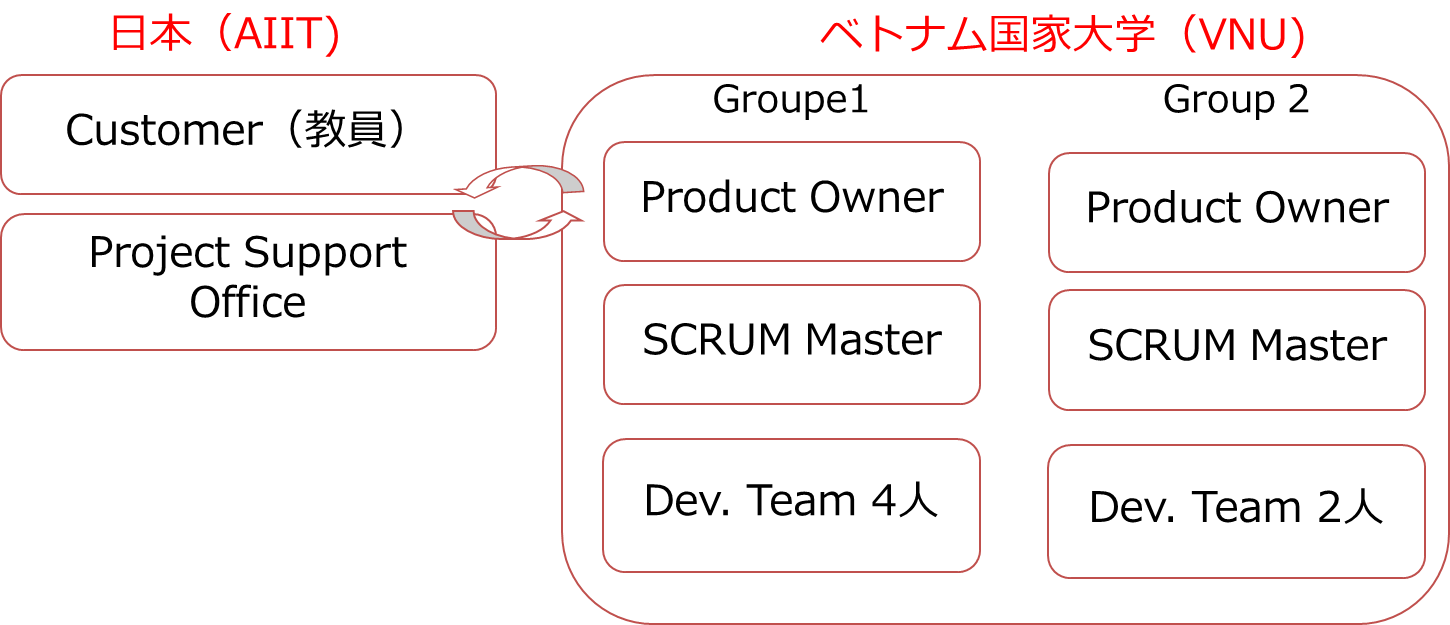
\includegraphics[width=\columnwidth]{./figures/PBL_organization.png}
    \caption{PBL organization}
    \label{fig:pblorganization}
  \end{center}
\end{figure}



\subsubsection{スケジュール}
本プロジェクトの開発フェーズのスケジュールは2012年7月1日から2012年8月30日までの2か月間である.
開発プロセスとスケジュールとしては,モデルに基づき,スプリントを3回,スプリント0(ゼロ)を組み込んだ.
スプリント期間は設計からテストまでを繰り返す.スプリントの長さは1週間とした(図\ref{fig:PBLSchedule}).
\begin{figure}[htb]
  \begin{center}
    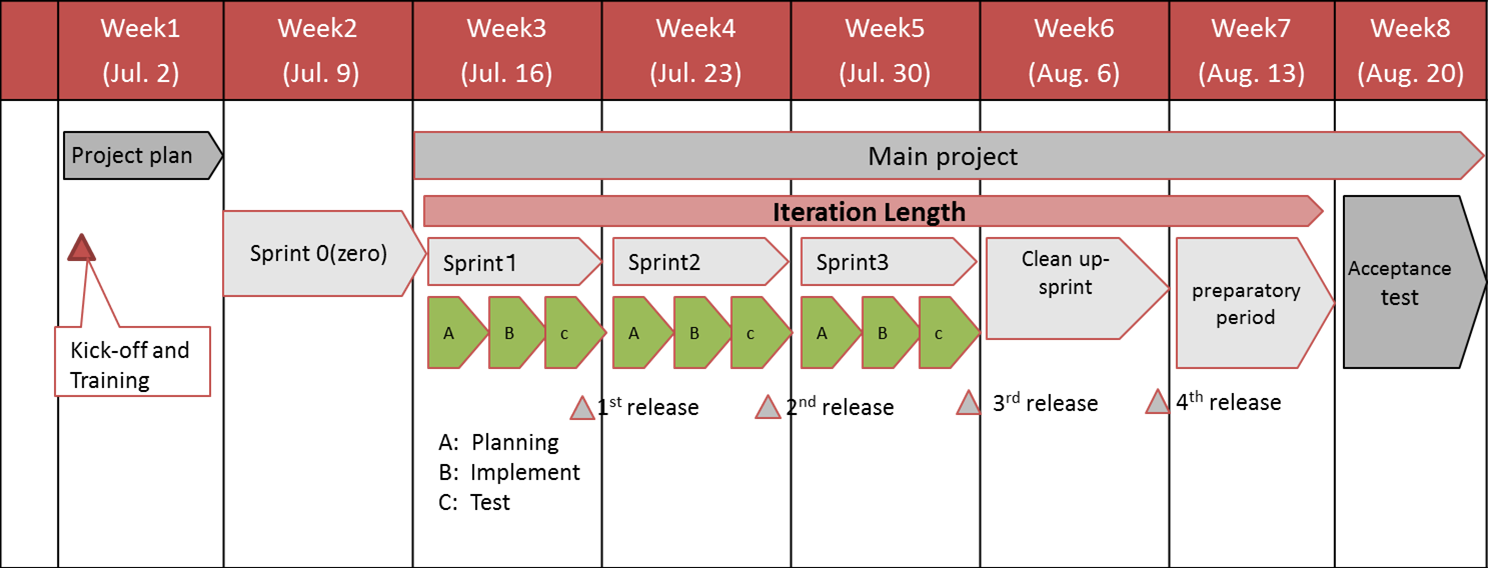
\includegraphics[width=\columnwidth]{./figures/PBLSchedule.png}
    \caption{PBL Schedule}
    \label{fig:PBLSchedule}
  \end{center}
\end{figure}

\subsubsection{要件定義}
顧客役のAIIT側の教員から示された要求仕様を基に,VNU側のプロダクトオーナーが作成した.

\subsubsection{スプリント計画}
プロダクトバックログを基に,VNU側の開発チームが作成した.
\subsubsection{プロジェクトのモニタリング}


毎週土曜日にAIIT側で進捗状況確認を実施する.最新のプロダクトバックログ,スプリントバックログ,バーンダウンチャートを共有することで,開発の進行状況を確認する,問題があればフォローした.
図\ref{fig:progresscheck}に,進捗状況のモニタリングに用いた物を示す.これはスプリント2回目の物である.

\begin{figure}[htb]
  \begin{center}
    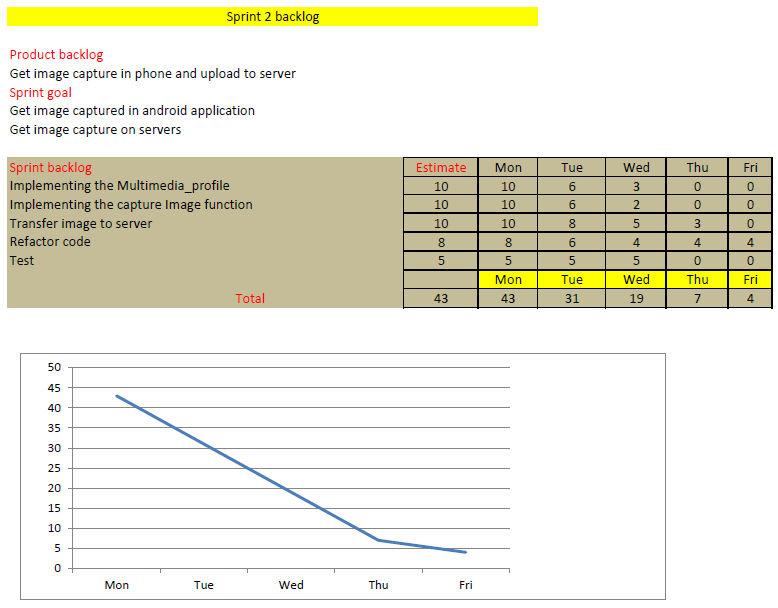
\includegraphics[width=\columnwidth]{./figures/Progress.png}
    \caption{VNU Sprint2 Progress Check}
    \label{fig:progresscheck}
  \end{center}
\end{figure}

そのほかにも,GitHub上で日々のソースコード更新作業がおなわれており,それに対して,コメントするといったコミュニケーションが行われていた(図図\ref{fig:dailyupdate}).

\begin{figure}[htb]
  \begin{center}
    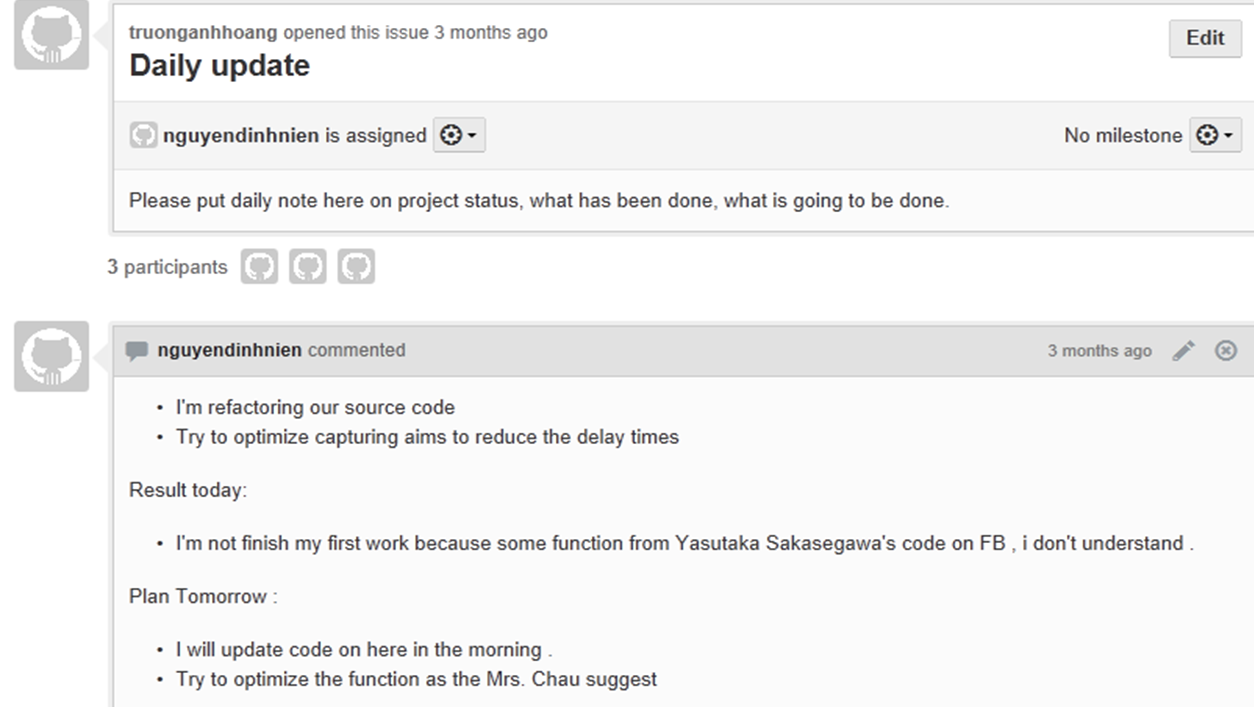
\includegraphics[width=\columnwidth]{./figures/DailyUPDate.png}
    \caption{DailyUpdate}
    \label{fig:dailyupdate}
  \end{center}
\end{figure}

\subsection{プロジェクトの実行結果}
\begin{description}
 \item[生産性] プロジェクトで新たに作成したJava言語の行数:745(SLOC).
 \item[品質] 受け入れテストの際,バグは発見されていない.
 \item[納期]スケジュール通り2012年8月30日にロボットサービスソフトウェアを顧客役のAIITの教員へ納品し,プロジェクトは無事完了した.
\end{description}
生産性については,PBLという教育プロジェクトの一面もあるため,比較は難しいが,品質については,受け入れ時にすべて機能に不具合が無いという,過去4年の国際PBLのプロジェクトの中で最も高い品質を示した.
また,
\begin{enumerate}
 \item 開発用の技術リファレンスが一部欠如していた.
 \item 開発ドキュメントの図の一部が日本語で書かれていた.
 \item 開発途中で開発機材のアンドロイドスマートフォンが故障した.
\end{enumerate}
などの課題が発生したにもかかわらず,期日通りにプロジェクトを完了させている.

\section{開発プロジェクトの経験から得た知見}\label{sec:lessonslearned}
\subsection{プロジェクトにおける振り返り}
開発プロジェクト終了後,我々は,VNUの学生にアンケートを実施した.
今回の開発プロジェクトの経験を通しての率直な意見を収集し,
良かった点と課題,改善点をまとめた.

まず,良かった点としては,次の点が挙げられた.

\begin{enumerate}
 \item スクラムプロセスは非常に柔軟性がある.
 \item 開発メンバ同士の作業の状態を明瞭にできた.
 \item スクラムがプロジェクトの透明性を高めた.
 \item SkypeやFacebook,Mailでのコミュニケーションにより,情報共有が円滑
       に行えた.
 \item GitHub等ソーシャル開発環境が開発効率を上げた.
\end{enumerate}

次に,課題として,次の点が挙げられた.

\begin{enumerate}
 \item 毎週の進捗管理とレポートは,開発者に負担がかかる.しかしレポートは必ず必要である.
 \item プロジェクトが期間短いため.開発に十分ではない.
 \item ディリースクラムは,毎日同じ時間,同じ場所で行うため,その際不在のメンバへの配慮が必要.
\end{enumerate}

最後に,改善が求められる点として以下の意見があった.

\begin{enumerate}
 \item 事前に様式を準備し配布しておくこと.
 \item 今回の開発プロジェクトで適用した技術や要求仕様が難しい.
 \item プロジェクト期間と事前の教育期間が短いため開発実施には十分ではない.
\end{enumerate}

また,国際PBLを実施したことの教育効果として,以下の点が指摘された.

\begin{enumerate}
 \item スクラムについての経験と実際のプロジェクトで作業する方法につい
       て学ぶことが出来た.
 \item チームワークやコミュニケーションは高品質のソフトウェアを開発する
       上で非常に重要であることを学んだ.
\end{enumerate}


\subsection{考察}

国際プロジェクトの課題として,言語が異なることによるコ
ミュニケーションの難しさと相対的な品質の低さを予想していた.
しかし,プロジェクト結果とアンケートの意見から,コミュニケーションは予
想より良好であった.
さらに,開発中は不具合修正も散見されたが受け入れテストの際は「全て機能が,顧客役のAIIT側の教員が期待したとおりに動作し不具合は一切無し」という品質を示した.これは,アジャイル開発手法スクラムを基にした,本モデルにコミュニケーションとフィードバックの機会を意図的に盛り込んだ効果といえよう.


迅速な開発スピードと柔軟性の両立については,開発スピードは今回は遅延無
くプロジェクトを完了できたことから,期待するスピードが得られたと考えて
良い.しかし,顧客からの要求事項の変化に強いかという点に関しては,事前
に要求仕様を提示したこともあり,今回のプロジェクトでは確認できなかっ
た.

PBLとして見た場合の教育効果として,高品質のソフトウェアを開発するための
チームワークとコミュニケーションを学ぶことができたという意見がアンケー
トの結果から得られ,これは大きな成果といえる.

%筆者らは,繰り返し型のプロセスにより,繰り返し学習を即す効果があると考えている.
さらに,普段の授業では体験できない,国際開発プロジェクトへの参画を通し
て,PBLのメンバには,異文化/異言語の相手とも積極的にコミュニケーション
をとる姿勢が見られるようになった.

\section{おわりに}\label{sec:concludion}
本論文では,ロボットのためのソフトウェア開発を迅速かつ安価に実施するた
めに,アジャイル開発手法Scrumとオフショア開発を組み合わせた国際開発プロ
ジェクトモデルを提案した.このモデルを,ロボットサービス開発をテーマと
したベトナムの学生との国際PBLに導入して検証したところ,ロボットサービス
開発においても品質が確保されたソフトウェアを短期間で作成できることがわ
かった.
Scrumは,1980年代の日本の製造業のノウハウを集約した開発プロセスが,米国で
体系化されたものである.これを再び,日本の主要な製造業であるロボットの
ためのサービスのソフトウェア開発に適用することでその有効性を示すことが
できた.

また,今回のPBLで明らかになった課題や改善点への対応を行い,ロボットサービ
スソフトウェア開発における標準的な開発プロセスの確立に向けて,本モデルを
洗練させていきたい. また,技術者教育の面からも,参加者に対する国際プロジェ
クト開発の学習効果がより向上するように,今後ともPBLでのトレーニングメソッ
ドとして改善を行っていく予定である.

%% 謝辞(ある場合のみ)
\section*{謝辞}
本プロジェクトに参加したベトナム国家大学の学生
Manh-Cuong NGUYEN氏, Duc-Kien DO氏, Dinh-Nien NGUYEN氏,
Khac-Phong DO氏,Hung-Quan TRAN氏, Xuan-Thuy DONG氏,
Dinh-Vuong PHAM氏, Manh-Toan NGUYEN氏,Xuan-Hoa NGO氏, Xuan-Thanh NGUYEN氏
に謝意を表します.

%% 文献
\bibliographystyle{junsrt}
\bibliography{reference}

\end{document}